\documentclass[10pt]{article}

% Cover spread size including print marks:
% 456mm x 233.2mm

\makeatletter

\RequirePackage{geometry}
\geometry{
  paperwidth=1292.598pt,
  paperheight=661.039pt,
}

\RequirePackage[portuguese]{babel}
\RequirePackage{xcolor}
\RequirePackage{graphicx}
\RequirePackage{eso-pic}

\RequirePackage{fontspec}
\defaultfontfeatures{ Ligatures={TeX}, Path = {./assets/fonts/}, }

\setmainfont[
  Numbers = Lining,
  SmallCapsFont = EBGaramondSC12-Regular.otf,
  ItalicFont = EBGaramond12-Italic.otf,
  BoldFont = Crimson-Bold.otf,
  BoldItalicFont = Crimson-BoldItalic.otf,
]{EBGaramond12-Regular.otf}

\graphicspath{{./assets/photos/300dpi/}}

\renewcommand\portuguesehyphenmins{{3}{3}}

\setlength{\parskip}{0pt}
\setlength{\parindent}{0pt}
\setlength{\fboxsep}{0pt}

\RequirePackage[final,babel=true]{microtype}

\makeatother

\hyphenation{Nyana-tiloka Nyana-ponika}

\begin{document}

\thispagestyle{empty}\mbox{}

\AddToShipoutPictureBG*{\put(0,0){%
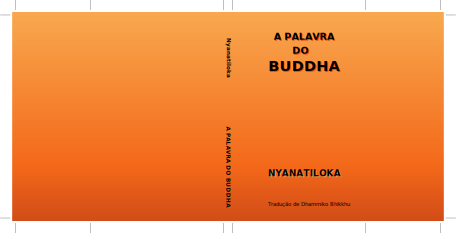
\includegraphics[width=\paperwidth]{palavra-do-buddha-cover.pdf}%
}}

\AddToShipoutPictureFG*{\put(\LenToUnit{20mm},\LenToUnit{20mm}){%
\begin{minipage}[b][175mm][t]{185pt}%
\fontsize{11.5}{16.5}\selectfont

Siddhārtha Gautama, o Buddha nasceu na cidade de Kapilavastu, hoje Nepal, em 563
a.C. Aos 29 anos de idade o príncipe Siddhārtha retirou-se da corte e dirigiu-se
para a floresta com o propósito de praticar ascese, até encontrar a razão e o
fim do sofrimento. Procurando o seu próprio caminho chegou à realização da
essência da verdade a que denominou “O Caminho do Meio”, meditando debaixo da
árvore bodhi, ao largo do Rio Nerañjara, a que hoje se chama Bodhgayā, no Estado
do Bhiar, Índia. Atingiu a iluminação na lua cheia de Maio de 528 a.C.,
tornando-se um Buddha, o Desperto, o que realizou a natureza de Buddhi,
inteligência luminosa. Ensinou e divulgou o seu Ensinamento até ao final dos
seus dias.

\end{minipage}%
}}

\AddToShipoutPictureFG*{\put(\LenToUnit{255.11pt+40.1pt},\LenToUnit{20mm}){%
\begin{minipage}[b][175mm][t]{105mm}%
\fontsize{14}{18}\selectfont

Embora possa servir como primeira introdução para o principiante, o
objectivo principal deste livro é oferecer ao leitor que já se encontra mais
ou menos familiarizado com as ideias fundamentais do Budismo, uma síntese
clara, autêntica e concisa dos seus diversos ensinamentos, no enquadramento
das “Quatro Nobres Verdades”, respectivamente as verdades do sofrimento
(inerente a toda a existência), da origem do sofrimento, da extinção do
sofrimento e do caminho que conduz à extinção do sofrimento. Verifica-se
pelo próprio conteúdo do livro como os ensinamentos do Buddha, em última
análise, convergem todos para uma realização final: a Libertação do
Sofrimento. Por essa razão se encontrava impressa na capa da primeira edição
em alemão, a seguinte passagem do \emph{Aṅguttara Nikāya}:

\bigskip

\emph{“Eu ensino não só a verdade do sofrimento, como também a libertação desse sofrimento.”}

\vfill

{\centering
\includegraphics[width=30mm]{sumedharama-logo-black-300dpi-w640.png}

\bigskip

\small
\emph{para distribuição gratuita}
\par}

\end{minipage}%
}}

\AddToShipoutPictureFG*{\put(\LenToUnit{1037.48pt+13.88pt},\LenToUnit{20mm}){%
\begin{minipage}[b][559pt][t]{185pt}%
\setlength{\parindent}{12pt}
\fontsize{9.5}{12.5}\selectfont

{\centering
  \includegraphics[width=26mm]{nyanatiloka-maha-thera.png}%
\par}

\bigskip

\noindent
O Venerável \textbf{Nyanatiloka Mahāthera} nasceu a 19~de fevereiro de 1878 em
Wiesbaden, Alemanha, com o nome de Anton Walther Florus Gueth.

Em 1903, na idade de 25 anos, Nyanatiloka visitou o Sri Lanka e, em seguida,
procedeu à Birmânia, onde ele foi ordenado como um monge budista Theravāda. Em
1904, ele recebeu ordenação superior na Birmânia antes de retornar ao Sri Lanka
onde estudou Pāli. Em 1905, Nyanaponika permaneceu com seu antigo mentor, o
pioneiro monástico britânico Ananda Metteyya. Em 1906, ele publicou seu primeiro
trabalho budista em alemão, \emph{Das Wort des Buddha} (\emph{A~Palavra do Buda},
publicado em Inglês em~1927).

Em 1911, fundou um mosteiro, Island Hermitage, para os monges ocidentais em
Dodanduwa.

Em 1914, com a eclosão da 1ª Guerra Mundial, Nyanatiloka foi detido pelos
britânicos no Sri Lanka, deportado para a Austrália (1915), libertado, viaja
para a China, é detido na China (assim que a China aderiu à guerra contra a
Alemanha), repatriado para a Alemanha em~1919.

Em 1920, após ter-lhe sido negada a reentrada no Sri Lanka, Nyanatiloka ensinou
em universidades japonesas por cinco anos. Em 1926, ele foi autorizado a
regressar a Island Hermitage.

Em 1939, com a declaração de guerra britânica contra a Alemanha nazista,
Nyanatiloka com outros alemães, foi novamente detido, primeiro no Sri Lanka e
depois na Índia (1941). Em 1948, foi autorizado a regressar ao Sri Lanka.

Em 1954 o Ven. Nyanatiloka e o Ven. Nyanaponika (um dos discípulos de
Nyanatiloka) foram os dois únicos monges nascidos no ocidente, convidados a
participar no Sexto Concílio Budista (Myanmar).

Morreu a 28 de maio de 1957, em Colombo, Sri Lanka, e foi-lhe dado um funeral de
estado.

\end{minipage}%
}}

\end{document}
